\documentclass{report}

\input{preamble}
\input{macros}
\input{letterfonts}

\title{\Huge{Magnet Precalculus CD}\\Vectors}
\author{\huge{Devin D. Droddy}}
\date{}

\begin{document}

\maketitle
\newpage% or \cleardoublepage
% \pdfbookmark[<level>]{<title>}{<dest>}
\pdfbookmark[section]{\contentsname}{toc}
\tableofcontents
\pagebreak

\chapter{Geometric Representation of Vectors}

\section{Combination }

\section{Magnitude of Vectors}

The magnitude (length) of a vector $v=\left\langle a,b \right\rangle$ is $||v||=\sqrt{a^2+b^2}$. If vector $v$ is represented by the arrow from $(x_1,y_1)$ to $(x_2,y_2)$, then $||v||=\sqrt{(x_2-x_1)^2+(y_2-y_1)^2}$.

\section{Unit Vector}

\dfn{Unit Vector}{
	A vector $u$ for which $||u||=1$ is called a \textbf{unit vector}.

	\begin{center}
		$u=\frac{v}{||v||}$

		$i=\left\langle 1,0 \right\rangle$ and $j=\left\langle 0,1 \right\rangle$
	\end{center}
}

\section{Components of a Vector}

Let $v$ be a vector with magnitude $||v||$ and direction $\theta$. Then, $v=\left\langle a,b \right\rangle=ai+bj$ where $a=||v||\cos(\theta)$ and $b=||v||\sin(\theta)$. Therefore, we can express $v$ as $v=||v||\cos(\theta)i+||v||\sin(\theta)j$

\chapter{The Language of Vectors}

\section{The Dot Product}

\dfn{Dot Product}{
	A \textbf{\ul{dot product}} of $u=\left\langle a_1,b_1 \right\rangle$ and $v=\left\langle a_2,b_2 \right\rangle$ is $u \bullet v=a_1a_2+b_1b_2$
}

Another form of the dot product is $u \bullet v=||u||||v||\cos(\theta)$, where $\theta$ is the angle between $u$ and $v$.\\

To find the angle between two vectors, the dot product can be used:

Let $\theta$ be the angle between two vectors, $u$ and $v$. Where $0\le\theta\le\pi$, $\cos(\theta)=\frac{u \bullet v}{||u||||v||}$\\

The dot product can be used to find the magnitude of a vector:

$u=\left\langle a,b \right\rangle;||u||=\sqrt{a^2+b^2}=\sqrt{(a \bullet a)+(b \bullet b)}=\sqrt{u \bullet u}=\sqrt{u^2}$

\dfn{Orthogonal Vectors}{
	When two angles are orthogonal (a.k.a. perpendicular or normal), their dot product is 0.
}

\qs{}{
	Find the angle between the vectors $u=2i-j$ and $v=6i+4j$
}

\sol $\cos(\theta)=\frac{(2 \bullet 6)+(-1 \bullet 4)}{\sqrt{2^2+(-1)^2}\bullet\sqrt{6^2+4^2}}=\frac{12-4}{\sqrt{5}\bullet\sqrt{52}}=\frac{8}{\sqrt{260}}=\frac{8}{2\sqrt{65}};\theta=\cos^{-1}(\frac{8}{1\sqrt{65}})\approx \boxed{60.255^\circ}$

\section{Projection of a Vector Onto Another}

The projection of one vector onto another can be thought of as finding the shadow that one casts on the other. Consider the following scenario:

\begin{center}
	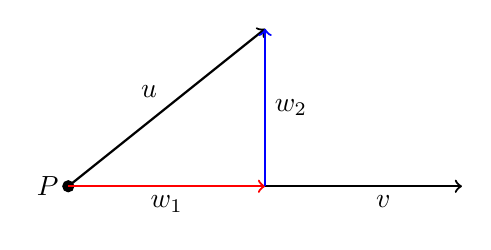
\begin{tikzpicture}
		\filldraw[black] (0,0) circle (2pt) node [anchor=east]{$P$};
		\draw[black, thick, ->] (0,0) -- (2.5, 2);
		\filldraw[black] (1.25,1) node [anchor=south east]{$u$};
		\draw[black, thick, ->] (0,0) -- (5,0);
		\filldraw[black] (4,0) node[anchor=north]{$v$};
		\draw[red, thick, ->] (0,0) -- (2.5,0);
		\filldraw[black] (1.25,0) node [anchor=north]{$w_1$};
		\draw[blue, thick, ->] (2.5,0) -- (2.5,2);
		\filldraw[black] (2.5,1) node [anchor=west]{$w_2$};
	\end{tikzpicture}
\end{center}

Here, vectors $u$ and $v$ start at the same point $P$. The projection of $u$ onto $v$ is $w_1$. If there were a light source pointing straight down, $w_1$ would the the shadow cast by $u$ on $v$. $w_2$ is defined as $u-w_1$, but by the nature of projection, it is also orthogonal to $v$.

Projection is represtented mathematically as $\proj_v(u)$, where $u$ is being projected onto $v$. $\proj_vu=(\frac{u \bullet v}{v^2})v$

\qs{}{Find $\proj_v(u)$ where $u=\left\langle 4,2 \right\rangle$ and $v=\left\langle 1,2 \right\rangle$}

\sol $\proj_v(u)=(\frac{u \bullet v}{v^2})v=\frac{(4 \bullet 1)+(2 \bullet 2)}{1^2+2^2}\left\langle 1,2 \right\rangle=\frac{4+4}{1+4}\left\langle 1,2 \right\rangle=\frac{8}{5}\left\langle 1,2 \right\rangle=\left\langle \frac{8}{5},\frac{16}{5} \right\rangle$
\begin{center}
	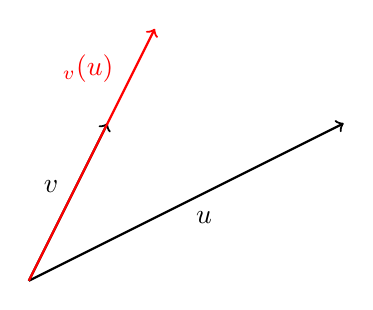
\begin{tikzpicture}
		\draw[black, thick, ->] (0,0) -- (1,2);
		\draw[black, thick, ->] (0,0) -- (4,2);
		\draw[red, thick, ->] (0,0) -- (8 / 5,16 / 5);
		\filldraw[red] (1.2,2.4) node [anchor=south east]{$\proj_v(u)$};
		\filldraw[black] (0.5,1) node [anchor=south east]{$v$};
		\filldraw[black] (2,1) node [anchor=north west]{$u$};
	\end{tikzpicture}
\end{center}

\end{document}